\chapter{Potpuna pretraga}

\key{Potpuna pretraga}
je opća metoda koja se može koristiti
za rješavanje gotovo svakog algoritamskog zadatka.
Ideja je grubom silom generirati sva moguća
rješenja zadatka,
a zatim odabrati najbolje rješenje ili prebrojiti
broj rješenja, ovisno o zadatku.

Potpuna pretraga je dobra tehnika
ako ima dovoljno vremena za prolazak kroz sva rješenja,
jer je pretragu obično lako implementirati
i uvijek daje ispravan odgovor.
Ako je potpuna pretraga prespora,
mogu biti potrebne druge tehnike, poput pohlepnih algoritama ili
dinamičkog programiranja.

\section{Generiranje podskupova}

\index{podskup}

Najprije razmotrimo zadatak generiranja
svih podskupova skupa od $n$ elemenata.
Na primjer, podskupovi skupa $\{0,1,2\}$ su
$\emptyset$, $\{0\}$, $\{1\}$, $\{2\}$, $\{0,1\}$,
$\{0,2\}$, $\{1,2\}$ i $\{0,1,2\}$.
Postoje dvije uobičajene metode za generiranje podskupova:
možemo provesti rekurzivnu pretragu
ili iskoristiti bitovni zapis cijelih brojeva.

\subsubsection{Metoda 1}

Elegantan način za prolazak kroz sve podskupove
nekog skupa jest korištenje rekurzije.
Sljedeća funkcija \texttt{search}
generira podskupove skupa
$\{0,1,\ldots,n-1\}$.
Funkcija održava vektor \texttt{subset}
koji će sadržavati elemente svakog podskupa.
Pretraga počinje kada se funkcija pozove
s parametrom 0.

\begin{lstlisting}
void search(int k) {
    if (k == n) {
        // obradi podskup
    } else {
        search(k+1);
        subset.push_back(k);
        search(k+1);
        subset.pop_back();
    }
}
\end{lstlisting}

Kada se funkcija \texttt{search}
pozove s parametrom $k$,
ona odlučuje hoće li
element $k$ uključiti u podskup ili ne,
a u oba slučaja
zatim poziva samu sebe s parametrom $k+1$.
Međutim, ako je $k=n$, funkcija uočava da su
svi elementi obrađeni
i da je podskup generiran.

Sljedeće stablo prikazuje pozive funkcije kada je $n=3$.
Uvijek možemo odabrati ili lijevu granu
($k$ nije uključen u podskup) ili desnu granu
($k$ je uključen u podskup).

\begin{center}
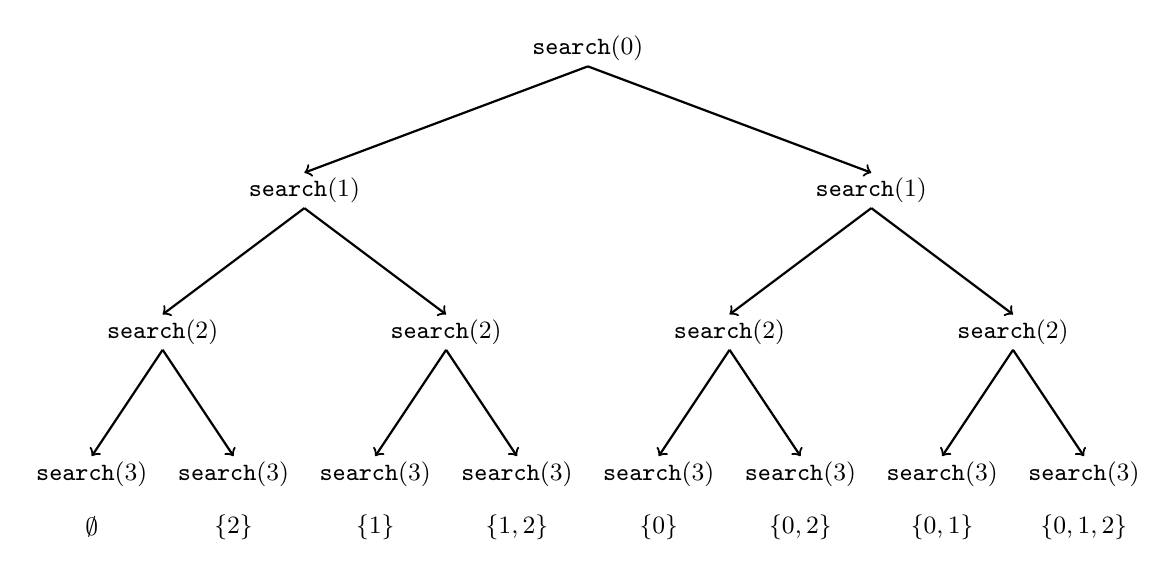
\begin{tikzpicture}[scale=.45]
  \begin{scope}
    \small
    \node at (0,0) {$\texttt{search}(0)$};

    \node at (-8,-4) {$\texttt{search}(1)$};
    \node at (8,-4) {$\texttt{search}(1)$};

    \path[draw,thick,->] (0,0-0.5) -- (-8,-4+0.5);
    \path[draw,thick,->] (0,0-0.5) -- (8,-4+0.5);

    \node at (-12,-8) {$\texttt{search}(2)$};
    \node at (-4,-8) {$\texttt{search}(2)$};
    \node at (4,-8) {$\texttt{search}(2)$};
    \node at (12,-8) {$\texttt{search}(2)$};

    \path[draw,thick,->] (-8,-4-0.5) -- (-12,-8+0.5);
    \path[draw,thick,->] (-8,-4-0.5) -- (-4,-8+0.5);
    \path[draw,thick,->] (8,-4-0.5) -- (4,-8+0.5);
    \path[draw,thick,->] (8,-4-0.5) -- (12,-8+0.5);

    \node at (-14,-12) {$\texttt{search}(3)$};
    \node at (-10,-12) {$\texttt{search}(3)$};
    \node at (-6,-12) {$\texttt{search}(3)$};
    \node at (-2,-12) {$\texttt{search}(3)$};
    \node at (2,-12) {$\texttt{search}(3)$};
    \node at (6,-12) {$\texttt{search}(3)$};
    \node at (10,-12) {$\texttt{search}(3)$};
    \node at (14,-12) {$\texttt{search}(3)$};

    \node at (-14,-13.5) {$\emptyset$};
    \node at (-10,-13.5) {$\{2\}$};
    \node at (-6,-13.5) {$\{1\}$};
    \node at (-2,-13.5) {$\{1,2\}$};
    \node at (2,-13.5) {$\{0\}$};
    \node at (6,-13.5) {$\{0,2\}$};
    \node at (10,-13.5) {$\{0,1\}$};
    \node at (14,-13.5) {$\{0,1,2\}$};


    \path[draw,thick,->] (-12,-8-0.5) -- (-14,-12+0.5);
    \path[draw,thick,->] (-12,-8-0.5) -- (-10,-12+0.5);
    \path[draw,thick,->] (-4,-8-0.5) -- (-6,-12+0.5);
    \path[draw,thick,->] (-4,-8-0.5) -- (-2,-12+0.5);
    \path[draw,thick,->] (4,-8-0.5) -- (2,-12+0.5);
    \path[draw,thick,->] (4,-8-0.5) -- (6,-12+0.5);
    \path[draw,thick,->] (12,-8-0.5) -- (10,-12+0.5);
    \path[draw,thick,->] (12,-8-0.5) -- (14,-12+0.5);
\end{scope}
\end{tikzpicture}
\end{center}

\subsubsection{Metoda 2}

Drugi način generiranja podskupova temelji se na
bitovnom zapisu cijelih brojeva.
Svaki podskup skupa od $n$ elemenata
može se prikazati kao niz od $n$ bitova,
što odgovara cijelom broju iz raspona $0 \ldots 2^n-1$.
Jedinice u nizu bitova označavaju
koji su elementi uključeni u podskup.

Uobičajena je konvencija da
posljednji bit odgovara elementu 0,
pretposljednji bit odgovara elementu 1,
i tako dalje.
Na primjer, bitovni zapis broja 25
jest 11001, što odgovara podskupu $\{0,3,4\}$.

Sljedeći kod prolazi kroz podskupove
skupa od $n$ elemenata

\begin{lstlisting}
for (int b = 0; b < (1<<n); b++) {
    // obradi podskup
}
\end{lstlisting}

Sljedeći kod pokazuje kako možemo pronaći
elemente podskupa koji odgovara nizu bitova.
Pri obradi svakog podskupa
kod gradi vektor koji sadrži
elemente tog podskupa.

\begin{lstlisting}
for (int b = 0; b < (1<<n); b++) {
    vector<int> subset;
    for (int i = 0; i < n; i++) {
        if (b&(1<<i)) subset.push_back(i);
    }
}
\end{lstlisting}

\section{Generiranje permutacija}

\index{permutacija}

Zatim razmotrimo zadatak generiranja
svih permutacija skupa od $n$ elemenata.
Na primjer, permutacije skupa $\{0,1,2\}$ su
$(0,1,2)$, $(0,2,1)$, $(1,0,2)$, $(1,2,0)$,
$(2,0,1)$ i $(2,1,0)$.
I ovdje postoje dva pristupa:
možemo koristiti rekurziju ili prolaziti kroz
permutacije iterativno.

\subsubsection{Metoda 1}

Kao i podskupovi, permutacije se mogu generirati
pomoću rekurzije.
Sljedeća funkcija \texttt{search} prolazi
kroz permutacije skupa $\{0,1,\ldots,n-1\}$.
Funkcija gradi vektor \texttt{permutation}
koji sadrži permutaciju,
a pretraga počinje kada se funkcija
pozove bez parametara.

\begin{lstlisting}
void search() {
    if (permutation.size() == n) {
        // obradi permutaciju
    } else {
        for (int i = 0; i < n; i++) {
            if (chosen[i]) continue;
            chosen[i] = true;
            permutation.push_back(i);
            search();
            chosen[i] = false;
            permutation.pop_back();
        }
    }
}
\end{lstlisting}

Svaki poziv funkcije dodaje novi element u
\texttt{permutation}.
Niz \texttt{chosen} označava koji su
elementi već uključeni u permutaciju.
Ako je veličina vektora \texttt{permutation} jednaka veličini skupa,
permutacija je generirana.

\subsubsection{Metoda 2}

\index{next\_permutation@\texttt{next\_permutation}}

Druga metoda za generiranje permutacija
jest započeti s permutacijom
$\{0,1,\ldots,n-1\}$ i opetovano
koristiti funkciju koja konstruira sljedeću permutaciju
po rastućem poretku.
Standardna biblioteka jezika C++ sadrži funkciju
\texttt{next\_permutation} koja se za to može koristiti:

\begin{lstlisting}
vector<int> permutation;
for (int i = 0; i < n; i++) {
    permutation.push_back(i);
}
do {
    // obradi permutaciju
} while (next_permutation(permutation.begin(),permutation.end()));
\end{lstlisting}

\section{Pretraga s vraćanjem}

\index{pretraga s vraćanjem}

Algoritam \key{pretrage s vraćanjem}
počinje s praznim rješenjem
i proširuje rješenje korak po korak.
Pretraga rekurzivno
prolazi kroz sve različite načine na koje se
rješenje može konstruirati.

\index{zadatak s kraljicama}

Kao primjer, razmotrimo zadatak
izračunavanja broja
načina na koje se $n$ kraljica može postaviti na
šahovsku ploču veličine $n \times n$ tako da
nikoje dvije kraljice ne napadaju jedna drugu.
Na primjer, kada je $n=4$,
postoje dva moguća rješenja:

\begin{center}
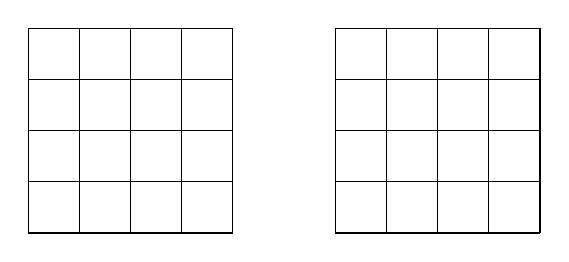
\begin{tikzpicture}[scale=.65]
  \begin{scope}
    \draw (0, 0) grid (4, 4);
    \node at (1.5,3.5) {\symqueen};
    \node at (3.5,2.5) {\symqueen};
    \node at (0.5,1.5) {\symqueen};
    \node at (2.5,0.5) {\symqueen};

    \draw (6, 0) grid (10, 4);
    \node at (6+2.5,3.5) {\symqueen};
    \node at (6+0.5,2.5) {\symqueen};
    \node at (6+3.5,1.5) {\symqueen};
    \node at (6+1.5,0.5) {\symqueen};

  \end{scope}
\end{tikzpicture}
\end{center}

Zadatak se može riješiti pretragom s vraćanjem
tako da kraljice postavljamo na ploču red po red.
Preciznije, na svaki redak bit će
postavljena točno jedna kraljica tako da nijedna kraljica ne napada
nijednu od prethodno postavljenih kraljica.
Rješenje je pronađeno kada je svih
$n$ kraljica postavljeno na ploču.

Na primjer, kada je $n=4$,
neka djelomična rješenja koja generira
algoritam pretrage s vraćanjem izgledaju ovako:

\begin{center}
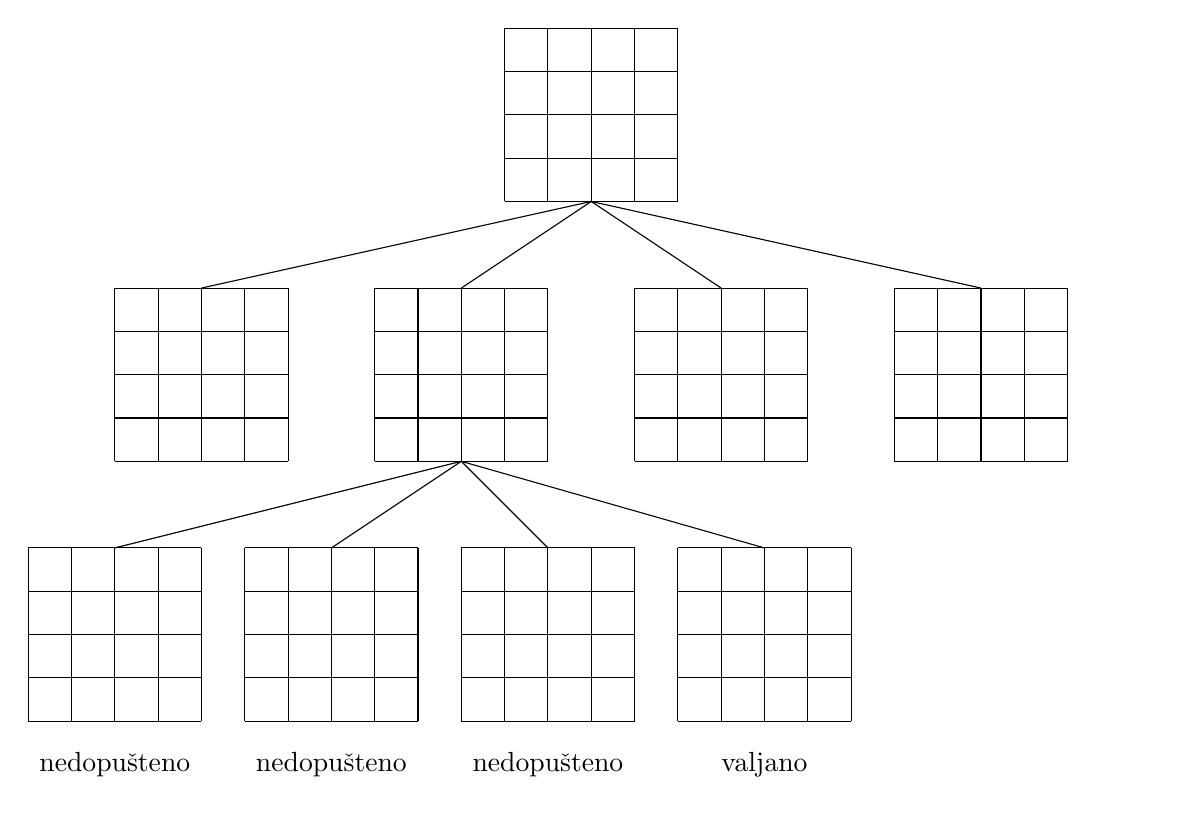
\begin{tikzpicture}[scale=.55]
  \begin{scope}
    \draw (0, 0) grid (4, 4);

    \draw (-9, -6) grid (-5, -2);
    \draw (-3, -6) grid (1, -2);
    \draw (3, -6) grid (7, -2);
    \draw (9, -6) grid (13, -2);

    \node at (-9+0.5,-3+0.5) {\symqueen};
    \node at (-3+1+0.5,-3+0.5) {\symqueen};
    \node at (3+2+0.5,-3+0.5) {\symqueen};
    \node at (9+3+0.5,-3+0.5) {\symqueen};

    \draw (2,0) -- (-7,-2);
    \draw (2,0) -- (-1,-2);
    \draw (2,0) -- (5,-2);
    \draw (2,0) -- (11,-2);

    \draw (-11, -12) grid (-7, -8);
    \draw (-6, -12) grid (-2, -8);
    \draw (-1, -12) grid (3, -8);
    \draw (4, -12) grid (8, -8);
    \draw[white] (11, -12) grid (15, -8);
    \node at (-11+1+0.5,-9+0.5) {\symqueen};
    \node at (-6+1+0.5,-9+0.5) {\symqueen};
    \node at (-1+1+0.5,-9+0.5) {\symqueen};
    \node at (4+1+0.5,-9+0.5) {\symqueen};
    \node at (-11+0+0.5,-10+0.5) {\symqueen};
    \node at (-6+1+0.5,-10+0.5) {\symqueen};
    \node at (-1+2+0.5,-10+0.5) {\symqueen};
    \node at (4+3+0.5,-10+0.5) {\symqueen};

    \draw (-1,-6) -- (-9,-8);
    \draw (-1,-6) -- (-4,-8);
    \draw (-1,-6) -- (1,-8);
    \draw (-1,-6) -- (6,-8);

    \node at (-9,-13) {nedopušteno};
    \node at (-4,-13) {nedopušteno};
    \node at (1,-13) {nedopušteno};
    \node at (6,-13) {valjano};

  \end{scope}
\end{tikzpicture}
\end{center}

Na najnižoj razini prve tri konfiguracije
su nedopuštene jer se kraljice međusobno napadaju.
Međutim, četvrta konfiguracija je valjana
i može se proširiti do potpunog rješenja
postavljanjem još dviju kraljica na ploču.
Postoji samo jedan način da se postave preostale dvije kraljice.

\begin{samepage}
Algoritam se može implementirati ovako:
\begin{lstlisting}
void search(int y) {
    if (y == n) {
        count++;
        return;
    }
    for (int x = 0; x < n; x++) {
        if (column[x] || diag1[x+y] || diag2[x-y+n-1]) continue;
        column[x] = diag1[x+y] = diag2[x-y+n-1] = 1;
        search(y+1);
        column[x] = diag1[x+y] = diag2[x-y+n-1] = 0;
    }
}
\end{lstlisting}
\end{samepage}
Pretraga počinje pozivom \texttt{search(0)}.
Veličina ploče je $n \times n$,
a kod broj rješenja računa
u varijablu \texttt{count}.

Kod pretpostavlja da su redci i stupci
ploče numerirani od 0 do $n-1$.
Kada se funkcija \texttt{search}
pozove s parametrom $y$,
ona postavlja kraljicu u redak $y$
i zatim poziva samu sebe s parametrom $y+1$.
Zatim, ako je $y=n$, rješenje je pronađeno
i varijabla \texttt{count} povećava se za jedan.

Niz \texttt{column} prati stupce
koji sadrže kraljicu,
a nizovi \texttt{diag1} i \texttt{diag2}
prate dijagonale.
Nije dopušteno dodati još jednu kraljicu u
stupac ili na dijagonalu koja već sadrži kraljicu. 
Na primjer, stupci i dijagonale
ploče $4 \times 4$ numerirani su ovako:

\begin{center}
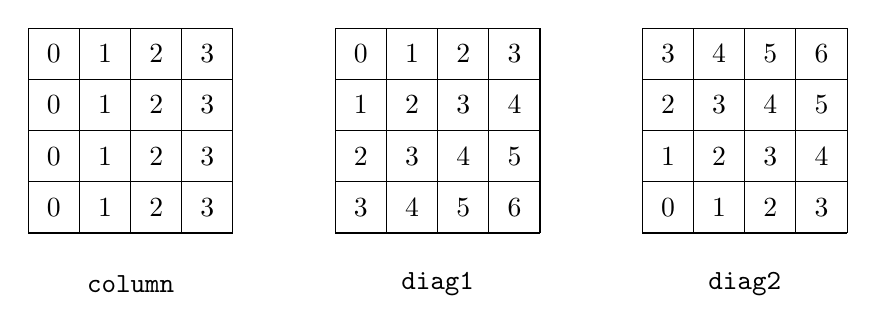
\begin{tikzpicture}[scale=.65]
  \begin{scope}
    \draw (0-6, 0) grid (4-6, 4);
    \node at (-6+0.5,3.5) {$0$};
    \node at (-6+1.5,3.5) {$1$};
    \node at (-6+2.5,3.5) {$2$};
    \node at (-6+3.5,3.5) {$3$};
    \node at (-6+0.5,2.5) {$0$};
    \node at (-6+1.5,2.5) {$1$};
    \node at (-6+2.5,2.5) {$2$};
    \node at (-6+3.5,2.5) {$3$};
    \node at (-6+0.5,1.5) {$0$};
    \node at (-6+1.5,1.5) {$1$};
    \node at (-6+2.5,1.5) {$2$};
    \node at (-6+3.5,1.5) {$3$};
    \node at (-6+0.5,0.5) {$0$};
    \node at (-6+1.5,0.5) {$1$};
    \node at (-6+2.5,0.5) {$2$};
    \node at (-6+3.5,0.5) {$3$};

    \draw (0, 0) grid (4, 4);
    \node at (0.5,3.5) {$0$};
    \node at (1.5,3.5) {$1$};
    \node at (2.5,3.5) {$2$};
    \node at (3.5,3.5) {$3$};
    \node at (0.5,2.5) {$1$};
    \node at (1.5,2.5) {$2$};
    \node at (2.5,2.5) {$3$};
    \node at (3.5,2.5) {$4$};
    \node at (0.5,1.5) {$2$};
    \node at (1.5,1.5) {$3$};
    \node at (2.5,1.5) {$4$};
    \node at (3.5,1.5) {$5$};
    \node at (0.5,0.5) {$3$};
    \node at (1.5,0.5) {$4$};
    \node at (2.5,0.5) {$5$};
    \node at (3.5,0.5) {$6$};

    \draw (6, 0) grid (10, 4);
    \node at (6.5,3.5) {$3$};
    \node at (7.5,3.5) {$4$};
    \node at (8.5,3.5) {$5$};
    \node at (9.5,3.5) {$6$};
    \node at (6.5,2.5) {$2$};
    \node at (7.5,2.5) {$3$};
    \node at (8.5,2.5) {$4$};
    \node at (9.5,2.5) {$5$};
    \node at (6.5,1.5) {$1$};
    \node at (7.5,1.5) {$2$};
    \node at (8.5,1.5) {$3$};
    \node at (9.5,1.5) {$4$};
    \node at (6.5,0.5) {$0$};
    \node at (7.5,0.5) {$1$};
    \node at (8.5,0.5) {$2$};
    \node at (9.5,0.5) {$3$};

    \node at (-4,-1) {\texttt{column}};
    \node at (2,-1) {\texttt{diag1}};
    \node at (8,-1) {\texttt{diag2}};

  \end{scope}
\end{tikzpicture}
\end{center}

Neka $q(n)$ označava broj načina
na koje se $n$ kraljica može postaviti na ploču $n \times n$.
Gornji algoritam pretrage s vraćanjem
govori nam da je, na primjer, $q(8)=92$.
Kada $n$ raste, pretraga brzo postaje spora
jer broj rješenja raste
eksponencijalno.
Na primjer, izračun vrijednosti $q(16)=14772512$
gornjim algoritmom već traje oko minutu
na modernom računalu\footnote{Nije poznat način za efikasan
izračun većih vrijednosti $q(n)$. Trenutni rekord je
$q(27)=234907967154122528$, izračunat 2016. godine \cite{q27}.}.

\section{Podrezivanje pretrage}

Pretragu s vraćanjem često možemo optimizirati
podrezivanjem stabla pretrage.
Ideja je algoritmu dodati ''inteligenciju''
tako da što prije uoči
ako se djelomično rješenje ne može proširiti
do potpunog rješenja.
Takve optimizacije mogu imati golem
učinak na efikasnost pretrage.

Razmotrimo zadatak
izračunavanja broja putova
u mreži $n \times n$ od gornjeg lijevog kuta
do donjeg desnog kuta takvih da
put posjećuje svaki kvadrat točno jednom.
Na primjer, u mreži $7 \times 7$
postoji 111712 takvih putova.
Jedan od putova izgleda ovako:

\begin{center}
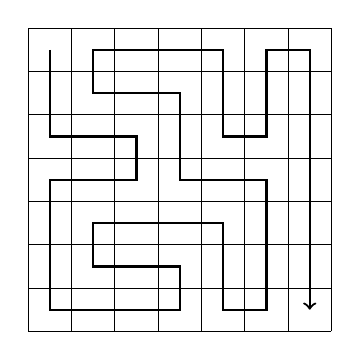
\begin{tikzpicture}[scale=.55]
  \begin{scope}
    \draw (0, 0) grid (7, 7);
    \draw[thick,->] (0.5,6.5) -- (0.5,4.5) -- (2.5,4.5) --
          (2.5,3.5) -- (0.5,3.5) -- (0.5,0.5) --
          (3.5,0.5) -- (3.5,1.5) -- (1.5,1.5) --
          (1.5,2.5) -- (4.5,2.5) -- (4.5,0.5) --
          (5.5,0.5) -- (5.5,3.5) -- (3.5,3.5) --
          (3.5,5.5) -- (1.5,5.5) -- (1.5,6.5) --
          (4.5,6.5) -- (4.5,4.5) -- (5.5,4.5) --
          (5.5,6.5) -- (6.5,6.5) -- (6.5,0.5);
  \end{scope}
\end{tikzpicture}
\end{center}

Usredotočit ćemo se na slučaj $7 \times 7$
jer je njegova razina težine primjerena našim potrebama.
Počinjemo s izravnim algoritmom pretrage s vraćanjem,
a zatim ga optimiziramo korak po korak koristeći zapažanja
o tome kako se pretraga može podrezati.
Nakon svake optimizacije mjerimo vrijeme izvođenja
algoritma i broj rekurzivnih poziva,
kako bismo jasno vidjeli učinak svake
optimizacije na efikasnost pretrage.

\subsubsection{Osnovni algoritam}

Prva verzija algoritma ne sadrži
nikakve optimizacije. Jednostavno koristimo pretragu s vraćanjem da generiramo
sve moguće putove od gornjeg lijevog kuta do
donjeg desnog kuta i prebrojimo takve putove.

\begin{itemize}
\item
vrijeme izvođenja: 483 sekunde
\item
broj rekurzivnih poziva: 76 milijardi
\end{itemize}

\subsubsection{Optimizacija 1}

U svakom rješenju prvi korak činimo
prema dolje ili prema desno.
Uvijek postoje dva puta koja 
su simetrična
s obzirom na dijagonalu mreže
nakon prvog koraka.
Na primjer, sljedeći putovi su simetrični:

\begin{center}
\begin{tabular}{ccc}
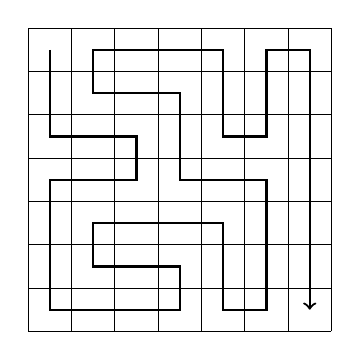
\begin{tikzpicture}[scale=.55]
  \begin{scope}
    \draw (0, 0) grid (7, 7);
    \draw[thick,->] (0.5,6.5) -- (0.5,4.5) -- (2.5,4.5) --
          (2.5,3.5) -- (0.5,3.5) -- (0.5,0.5) --
          (3.5,0.5) -- (3.5,1.5) -- (1.5,1.5) --
          (1.5,2.5) -- (4.5,2.5) -- (4.5,0.5) --
          (5.5,0.5) -- (5.5,3.5) -- (3.5,3.5) --
          (3.5,5.5) -- (1.5,5.5) -- (1.5,6.5) --
          (4.5,6.5) -- (4.5,4.5) -- (5.5,4.5) --
          (5.5,6.5) -- (6.5,6.5) -- (6.5,0.5);
  \end{scope}
\end{tikzpicture}
& \hspace{20px}
& 
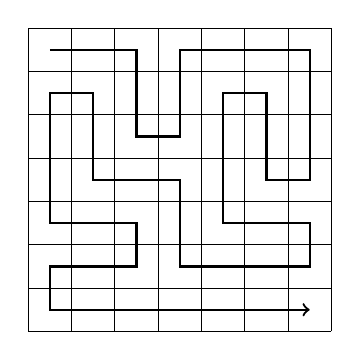
\begin{tikzpicture}[scale=.55]
  \begin{scope}[yscale=1,xscale=-1,rotate=-90]
    \draw (0, 0) grid (7, 7);
    \draw[thick,->] (0.5,6.5) -- (0.5,4.5) -- (2.5,4.5) --
          (2.5,3.5) -- (0.5,3.5) -- (0.5,0.5) --
          (3.5,0.5) -- (3.5,1.5) -- (1.5,1.5) --
          (1.5,2.5) -- (4.5,2.5) -- (4.5,0.5) --
          (5.5,0.5) -- (5.5,3.5) -- (3.5,3.5) --
          (3.5,5.5) -- (1.5,5.5) -- (1.5,6.5) --
          (4.5,6.5) -- (4.5,4.5) -- (5.5,4.5) --
          (5.5,6.5) -- (6.5,6.5) -- (6.5,0.5);
  \end{scope}
\end{tikzpicture}
\end{tabular}
\end{center}

Stoga možemo odlučiti da uvijek prvo
napravimo korak prema dolje (ili prema desno),
a na kraju broj rješenja pomnožimo s dva.

\begin{itemize}
\item
vrijeme izvođenja: 244 sekunde
\item
broj rekurzivnih poziva: 38 milijardi
\end{itemize}

\subsubsection{Optimizacija 2}

Ako put dođe do donjeg desnog kvadrata
prije nego što je posjetio sve ostale kvadrate mreže,
jasno je da
rješenje neće biti moguće dovršiti.
Primjer toga je sljedeći put:

\begin{center}
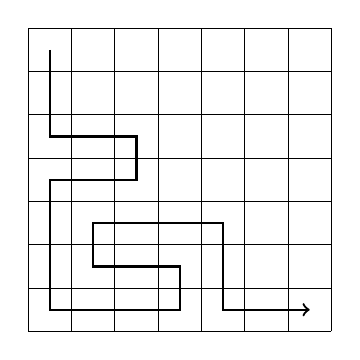
\begin{tikzpicture}[scale=.55]
  \begin{scope}
    \draw (0, 0) grid (7, 7);
    \draw[thick,->] (0.5,6.5) -- (0.5,4.5) -- (2.5,4.5) --
          (2.5,3.5) -- (0.5,3.5) -- (0.5,0.5) --
          (3.5,0.5) -- (3.5,1.5) -- (1.5,1.5) --
          (1.5,2.5) -- (4.5,2.5) -- (4.5,0.5) --
          (6.5,0.5);
  \end{scope}
\end{tikzpicture}
\end{center}
Koristeći to zapažanje, pretragu možemo odmah prekinuti
ako prerano dođemo do donjeg desnog kvadrata.
\begin{itemize}
\item
vrijeme izvođenja: 119 sekundi
\item
broj rekurzivnih poziva: 20 milijardi
\end{itemize}

\subsubsection{Optimizacija 3}

Ako put dodirne zid
i može skrenuti ili lijevo ili desno,
mreža se dijeli na dva dijela
koja sadrže neposjećene kvadrate.
Na primjer, u sljedećoj situaciji
put može skrenuti ili lijevo ili desno:

\begin{center}
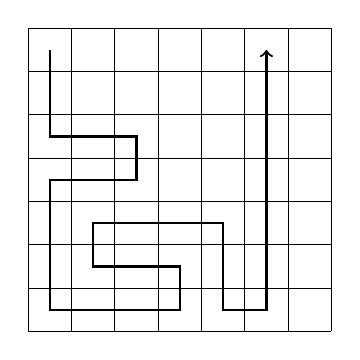
\begin{tikzpicture}[scale=.55]
  \begin{scope}
    \draw (0, 0) grid (7, 7);
    \draw[thick,->] (0.5,6.5) -- (0.5,4.5) -- (2.5,4.5) --
          (2.5,3.5) -- (0.5,3.5) -- (0.5,0.5) --
          (3.5,0.5) -- (3.5,1.5) -- (1.5,1.5) --
          (1.5,2.5) -- (4.5,2.5) -- (4.5,0.5) --
          (5.5,0.5) -- (5.5,6.5);
  \end{scope}
\end{tikzpicture}
\end{center}
U tom slučaju više ne možemo posjetiti sve kvadrate,
pa pretragu možemo prekinuti.
Ova optimizacija je vrlo korisna:

\begin{itemize}
\item
vrijeme izvođenja: 1.8 sekundi
\item
broj rekurzivnih poziva: 221 milijun
\end{itemize}

\subsubsection{Optimizacija 4}

Ideja Optimizacije 3
može se poopćiti:
ako put ne može nastaviti naprijed,
ali može skrenuti ili lijevo ili desno,
mreža se dijeli na dva dijela
koja oba sadrže neposjećene kvadrate.
Na primjer, razmotrimo sljedeći put:

\begin{center}
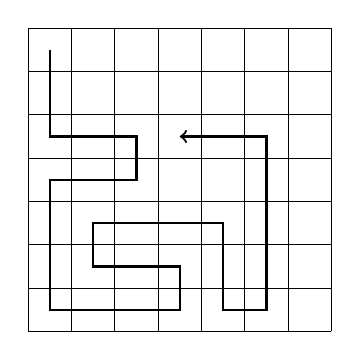
\begin{tikzpicture}[scale=.55]
  \begin{scope}
    \draw (0, 0) grid (7, 7);
    \draw[thick,->] (0.5,6.5) -- (0.5,4.5) -- (2.5,4.5) --
          (2.5,3.5) -- (0.5,3.5) -- (0.5,0.5) --
          (3.5,0.5) -- (3.5,1.5) -- (1.5,1.5) --
          (1.5,2.5) -- (4.5,2.5) -- (4.5,0.5) --
          (5.5,0.5) -- (5.5,4.5) -- (3.5,4.5);
  \end{scope}
\end{tikzpicture}
\end{center}
Jasno je da više ne možemo posjetiti sve kvadrate,
pa pretragu možemo prekinuti.
Nakon ove optimizacije pretraga je
vrlo efikasna:

\begin{itemize}
\item
vrijeme izvođenja: 0.6 sekundi
\item
broj rekurzivnih poziva: 69 milijuna
\end{itemize}

~\\
Sada je dobar trenutak da prestanemo optimizirati
algoritam i pogledamo što smo postigli.
Vrijeme izvođenja izvornog algoritma
bilo je 483 sekunde,
a sada, nakon optimizacija,
vrijeme izvođenja iznosi samo 0.6 sekundi.
Dakle, algoritam je nakon optimizacija postao
gotovo 1000 puta brži.

To je uobičajena pojava kod pretrage s vraćanjem
jer je stablo pretrage obično veliko
i već jednostavna zapažanja mogu učinkovito
podrezati pretragu.
Osobito su korisne optimizacije koje
nastupaju tijekom prvih koraka algoritma,
tj. pri vrhu stabla pretrage.

\section{Susret u sredini}

\index{susret u sredini}

\key{Susret u sredini} je tehnika
u kojoj se prostor pretrage dijeli na
dva dijela približno jednake veličine.
Za svaki od tih dijelova
provodi se zasebna pretraga,
a na kraju se rezultati pretraga kombiniraju.

Tehnika se može koristiti
ako postoji efikasan način za kombiniranje
rezultata pretraga.
U takvoj situaciji dvije pretrage mogu zahtijevati manje
vremena nego jedna velika pretraga.
Tipično, tehnikom susreta u sredini možemo
faktor $2^n$ pretvoriti
u faktor $2^{n/2}$.

Kao primjer, razmotrimo zadatak u kojem
nam je zadana lista od $n$ brojeva i
broj $x$,
a želimo utvrditi je li moguće
iz liste odabrati neke brojeve tako da
njihova suma bude $x$.
Na primjer, za listu $[2,4,5,9]$ i $x=15$
možemo odabrati brojeve $[2,4,9]$ i dobiti $2+4+9=15$.
Međutim, ako je $x=10$ za istu listu,
takvu sumu nije moguće formirati.

Jednostavan algoritam za taj zadatak jest
proći kroz sve podskupove elemenata i
provjeriti je li suma nekog od podskupova jednaka $x$.
Vrijeme izvođenja takvog algoritma je $O(2^n)$
jer postoji $2^n$ podskupova.
Međutim, tehnikom susreta u sredini
možemo postići efikasniji algoritam složenosti $O(2^{n/2})$\footnote{Ovu
su ideju 1974. godine uveli E. Horowitz i S. Sahni \cite{hor74}.}.
Uočimo da su $O(2^n)$ i $O(2^{n/2})$ različite
složenosti jer je $2^{n/2}$ jednako $\sqrt{2^n}$.

Ideja je podijeliti listu na
dvije liste $A$ i $B$ tako da obje
liste sadrže otprilike polovicu brojeva.
Prva pretraga generira sve podskupove
liste $A$ i pohranjuje njihove sume u listu $S_A$.
Odgovarajuće, druga pretraga stvara
listu $S_B$ iz liste $B$.
Nakon toga dovoljno je provjeriti je li moguće
odabrati jedan element iz $S_A$ i drugi
element iz $S_B$ tako da njihova suma bude $x$.
To je moguće točno onda kada postoji način da se
suma $x$ formira pomoću brojeva izvorne liste.

Na primjer, pretpostavimo da je lista $[2,4,5,9]$ i $x=15$.
Najprije listu dijelimo na $A=[2,4]$ i $B=[5,9]$.
Nakon toga stvaramo liste
$S_A=[0,2,4,6]$ i $S_B=[0,5,9,14]$.
U ovom slučaju sumu $x=15$ moguće je formirati
jer $S_A$ sadrži sumu $6$,
$S_B$ sadrži sumu $9$, a $6+9=15$.
To odgovara rješenju $[2,4,9]$.

Algoritam možemo implementirati tako da
njegova vremenska složenost bude $O(2^{n/2})$.
Najprije generiramo \emph{sortirane} liste $S_A$ i $S_B$,
što se može napraviti u $O(2^{n/2})$ vremenu tehnikom sličnom spajanju.
Nakon toga, budući da su liste sortirane,
možemo u $O(2^{n/2})$ vremenu provjeriti može li se
suma $x$ dobiti iz $S_A$ i $S_B$.